\documentclass[12pt]{scrartcl}
\usepackage[german, ngerman]{babel}
\usepackage{graphicx}
\usepackage{color}
\usepackage{url}
\usepackage{xcolor}
\usepackage{listings}
\usepackage{hyperref}
\usepackage{nameref}
\usepackage{varioref}
\hypersetup{
    colorlinks=true,
    linkcolor={black!50!black},
    % linkcolor={red!50!black},
    citecolor={black!50!black},
    urlcolor={black!50!black}
}
\usepackage[headsepline,footsepline]{scrlayer-scrpage}
\usepackage{biblatex}
\usepackage{amsmath}
\usepackage{float}

\newcommand{\code}[1]{\texttt{#1}}


\definecolor{mGreen}{rgb}{0,0.6,0}
\definecolor{mGray}{rgb}{0.5,0.5,0.5}
\definecolor{mPurple}{rgb}{0.58,0,0.82}
\definecolor{backgroundColour}{rgb}{0.95,0.95,0.95} %{cmyk}{0.05,0.05,0.05,0.05}

\lstdefinestyle{CStyle}{
    backgroundcolor=\color{backgroundColour},
    commentstyle=\color{mGreen},
    keywordstyle=\color{blue},
    numberstyle=\tiny\color{mGray},
    stringstyle=\color{mPurple},
    basicstyle=\footnotesize,
    breakatwhitespace=false,
    breaklines=true,
    captionpos=b,
    keepspaces=true,
    numbers=left,
    numbersep=5pt,
    showspaces=false,
    showstringspaces=false,
    showtabs=false,
    tabsize=2,
    language=C++
}

\lstdefinestyle{Terminal}{
    backgroundcolor=\color{backgroundColour},
    commentstyle=\color{black},
    keywordstyle=\color{black},
    numberstyle=\tiny\color{black},
    stringstyle=\color{black},
    basicstyle=\footnotesize,
    breakatwhitespace=false,
    breaklines=true,
    captionpos=b,
    keepspaces=true,
    numbers=none,
    numbersep=5pt,
    showspaces=false,
    showstringspaces=false,
    showtabs=false,
    tabsize=2,
}


\pagestyle{scrheadings}
\clearscrheadfoot
%\cfoot{Tobias Gruber}
\cfoot{\pagemark}
\chead{\headmark}
\automark[subsection]{section}


\begin{document}


\begin{titlepage}
    \vfill
	\centering
    \vspace{1.5cm}

	{\scshape\LARGE Hochschule München \par}
    {\scshape\Large Fakultät für Informatik und Mathematik\par}
	\vspace{1.5cm}




    \vfill
    {\LARGE\bfseries Praktikumsaufgabe 4 \\}
    \vspace{0.5cm}
	{in der Vorlesung\\}
    \vspace{0.5cm}
    {\LARGE\bfseries Computational Geometry\\~\\ \par}
	{\LARGE Konvexe Hüllen mit qhull\\~\\ \par}
	\vfill
    \vfill


    \begin{tabular}{ll}
    \normalsize
    Team:  & Christopher Hinz, Tobias Gruber\\
    Studiengruppe: & Master Informatik\\
    Studiensemester: & 1. Semester\\
    Schwerpunkt: & Embedded Computing\\
    \end{tabular}
    \vspace{1.5cm}

    \today

    \vspace{0.5cm}

    Sommersemester 2022

	\vfill

\end{titlepage}

\newpage

%%%%%%%%%%%%%%%%%%%%%%%%%%%%%
% Problemstellung
%%%%%%%%%%%%%%%%%%%%%%%%%%%%%
\section{Einführung}
Installieren Sie das Programm qhull, erzeugen Sie zufällige Punktmengen und berechnen Sie mit qhull konvexe Hüllen, auch in höheren Dimensionen (qhull bringt ein Werkzeug zur Erzeugung von Punktmengen mit). Plotten Sie die Zeiten für zunehmende Punktanzahlen bei unterschiedlichen Dimensionen (2-8). Versuchen Sie, die Ausgaben von qhull bei "geschwätzigster" Einstellung nachzuvollziehen, zu verstehen und ggf. mit Inhalten dieser Lehrveranstaltung in Einklang zu bringen.

\section{Benötigte Funktionen von qhull}

Qhull bietet 6 verschiedene Programme an:
\begin{itemize}
    \setlength\itemsep{0em}
    \item qconvex: convex hulls
    \item qdelaunay: Delaunay triangulations and furthest-site Delaunay triangulations
    \item qhalf: halfspace intersections about a point
    \item qhull: all structures with additional options
    \item qvoronoi: Voronoi diagrams and furthest-site Voronoi diagrams
    \item rbox: generate point distributions for qhull
\end{itemize}

Im Zuge dieses Praktikums werden wir sowohl rbox, zur Erzeugung von Punktmengen nutzen, als auch qconvex, zur Berechnen der konvexe Hüllen, nutzen.

\subsection{rbox (http://www.qhull.org/html/rbox.htm)}
Das Programm rbox generiert zufällige oder reguläre Punkte. Standardmäßig innerhalb eines Würfels (es sei denn die Optionen 's', 'x', oder 'y' werden übergeben).
Einige Beispiele zur Erzeugung von Punktmengen sind:
\begin{itemize}
    \setlength\itemsep{0em}
    \item rbox 10 D3: erzeugt 10 Punkte in 3D
    \item rbox 15 D4: erzeugt 15 Punkte in 4D
    \item rbox 10 D2: erzeugt 10 Punkte auf einem 2D Kreis
    \item rbox 100 W0: erzeugt 100 Punkte  auf der Oberfläche eines Würfels
\end{itemize}


\subsection{qconvex (http://www.qhull.org/html/qconvex.htm)}



Konvexe Hülle berechnen:
\begin{itemize}
    \item qconvex s < data: s = print summary, data = input data from file
\end{itemize}
\ \\


Punktmengen erzeugen und Konvexe Hülle plotten:
\begin{itemize}
    \item rbox 10 D3 | qconvex s: 10 Punkte in 3D und konvexe Hülle
\end{itemize}


TODO:
 wie geht plotten mit geomview (ist bereits installiert)?

\newpage

\section{Ergebnisse}


\section{Verifikation und Validierung}


%\begin{figure}[ht]
%    \centering
%    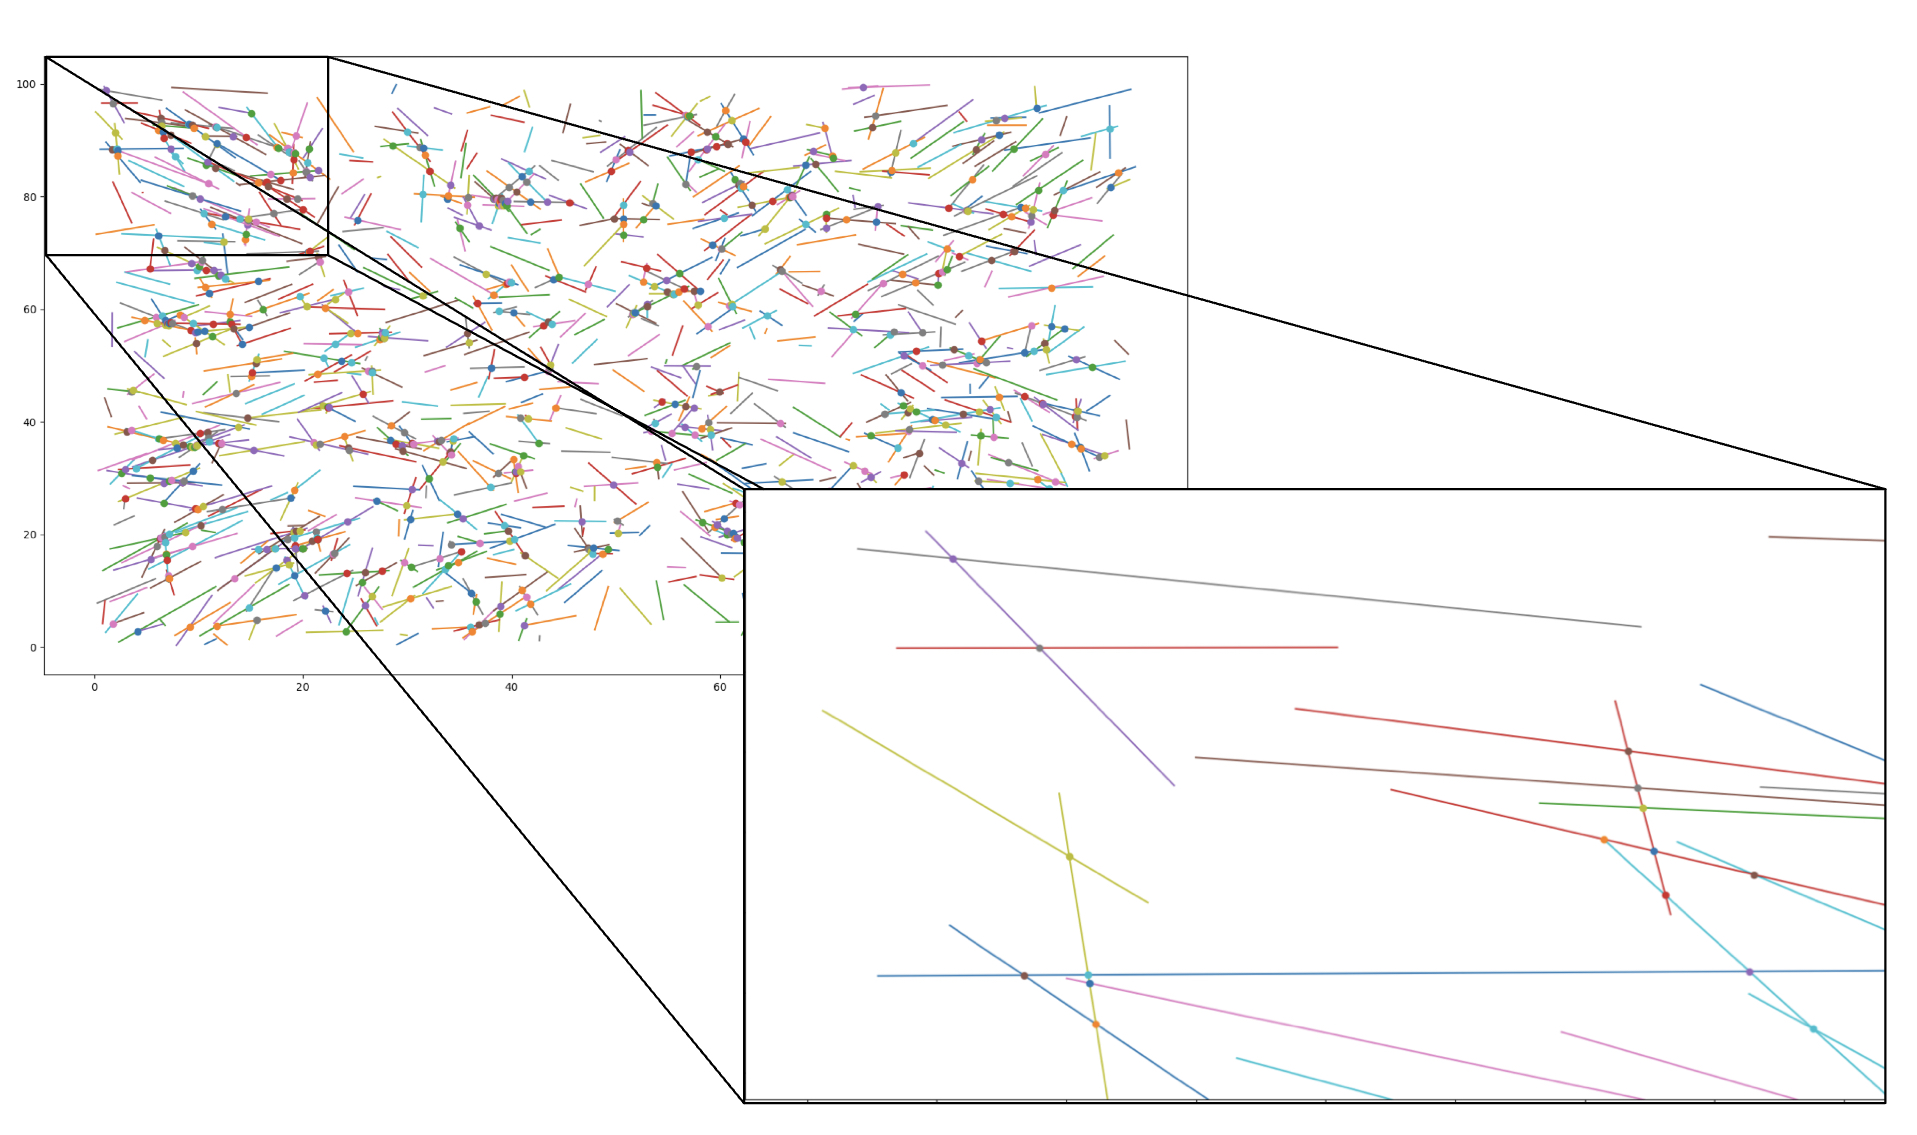
\includegraphics[scale=0.25]{Plot_zoom_and_all.jpeg}
%\end{figure}

%\begin{lstlisting}[style=Terminal, caption={testing.cpp: Ausgabe Konsole},captionpos=b, label={lst:ausgabe_test}]
%\end{lstlisting}



\end{document}
